\documentclass[10pt,twocolumn]{article}
\usepackage{epstopdf}
\usepackage{xspace}
\usepackage{amsmath}
\usepackage{slashed}
\def\ssWW{\ensuremath{ W^{\pm}W^{\pm}jj }\xspace}
\def\ts{\ensuremath{ \theta^{*} }\xspace}
\def\cts{\ensuremath{ cos(\ts) }\xspace}
\def\ctsnb{\ensuremath{ cos(\ts }\xspace}
\def\ctsSq{\ensuremath{ cos^{2}(\ts) }\xspace}
\def\ctsSqnb{\ensuremath{ cos^{2}(\ts) }\xspace}
\def\dR{\ensuremath{ \Delta R }\xspace}
\def\pt{\ensuremath{ p_T }\xspace}

\usepackage{graphicx}
\usepackage{color}
\usepackage{grffile}



\begin{document}
\begin{abstract}The unitarization of the longitudinal Vector Boson Scattering (VBS) cross section by the Higgs boson is a fundamental prediction of the Standard Model which has not been experimentally verified. In the first LHC run, ATLAS and CMS presented the first studies of VBS in events with two leptonically decaying same sign W bosons produced in association with two jets~\cite{a,b}. This VBS channel has the advantage of having small background contributions and yet a detectable rate compared to other VBS channels. However, the two neutrinos in the final state make full kinematic event reconstruction and hence evaluation the longitudinal scattering fraction difficult. The angular distributions of the leptons in the W boson rest frame, which are commonly used to fit polarization fractions, are not readily available due to the missing information resulting from the unmeasured neutrinos. In this paper we present a method to circumvent this problem by using deep machine learning to recover the angular distributions from measurable event kinematics, and compare sensitivities to longitudinal vector boson scattering with more traditional methods.
\end{abstract}

\section{Introduction}


The discovery of the Higgs-like boson at the
LHC~\cite{ATLAS_higgs,CMS_higgs}, was the first step toward
determining the properties of electroweak symmetry breaking
(EWSB). One important, and unverified, prediction of the Standard
Model is that the scattering amplitude of longitudinal vector bosons
($V_{L}V_{L} \rightarrow V_{L}V_{L}$) is unitarized by the Higgs
boson. Measuring VBS processes at a hadron collider, however, is
experimentally challenging. Currently, the ATLAS and CMS
collaborations have only been able study the W+,W+,jj final
state~\cite{ATLAS_ssWW,CMS_ssWW}. This final state with two same sign
leptons has the advantage of relatively small background from other
standard model processes including ``strong'' production which
dominates other VBS/VBF process. While an ideal candidate for
observing VBS, measuring the longitudinal fraction of these events is
not straight froward. In general the polarization of a gauge boson can
be determined from the angular distribution of its decay
products~\cite{?}. For a leptonic W the differential cross section can
be written in terms of polarization fractions as

%\begin{equation}
\begin{multline}
 \frac{1}{\sigma} \frac{d\sigma}{d\cts} = \frac{3}{8} f_L (1 \mp \cts)^2 + \frac{3}{8} f_R (1 \pm \cts)^2 \\ 
+\frac{3}{4} f_0 (1 - \ctsSq)  
\end{multline}
%\end{equation}
%  R. Ellis, W. Stirling, and B. Webber,
%QCD and collider
%physics
%, Camb. Monogr. Part. Phys. Nucl. Phys.
%Cosmol.
%8
%(1996) 1



Where \ts is the angle in the W's rest frame between the charged lepton and the W's direction in the lab frame. However, because of two neutrinos in the final state the W's rest frame cannot be directly measured. Do to these issues many proposals have been made to measure Longitudinal fractions in different final states, such as semileptonic WW~\cite{Han:2009em}, or ZZ (le houche report), however, these channel suffer from large backgrounds not present in the W+W+jj channel.  However, due to advantages of the same sign WW state attempts have been made to gain sensitivity through other variables than \ts. Doroba et.al. has show that the variable $R_{pt}=\frac{Ptl1*ptl2}{ptj1,ptj2}$  is sensitive to the longitudinal fraction in the W+W+jj final state \cite{Doroba:2012pd}.  It is natural to assume that all of the sensitivity to longitudinal scattering is not encompassed in a single variable, and that better discrimination could be obtained by combining all the event information with a machine learning technique. Thus the authors have developed a method using a neural network to map measurable quantities to the \cts distribution that contains the polarization information of the W boson. 



\section{Machine learning model}


While it has become common practice in high energy physics to use multi-variate techniques to separate signal 
from background, to the author's knowledge multi-variate regression has not been used to directly predict underlying quantities. 


For our purpose the goal of the multi-variate technique is to find the best mapping from the 14 measurable quantities (2 Leptons and 2 Jets each with $\pt,\eta,\phi$, and $\slashed{E}, \phi, E_{t}$) to the two values of \cts (one for each W) present in each event. Do to recent success with deep learn in other areas of HEP~\cite{Baldi:2014pta,Baldi:2014pta}. We choose a multi-layer neural network with a final output layer with linear activation. The neural network was implemented with the Theano software packages. Hyperparameters were roughly tuned by hand, but undoubtedly could be improved. The cost function was defined as the mean error squared and stochastic gradient descent was used to train the sample.
\small
\begin{equation}
F=-\sum_{i=1}^{n} [(\ctsnb_{1,i})-N_{1,i})^2+(\ctsnb_{2,i})-N_{2,i})^2]/n
\end{equation}
\normalsize
Where $\ctsnb_{1/2,i})$ is true value of \cts for each W boson with random ordering for $i$-th event, and $N_{1,2/i}$ is the value of the two output layers. 

Training events were split into three categorizes. 1/4 of the events where used in a training sample, 1/4 were used as a validation test against over training, and the remaining 1/2. were used to build templates and do sensitivities studies. 


\begin{figure}
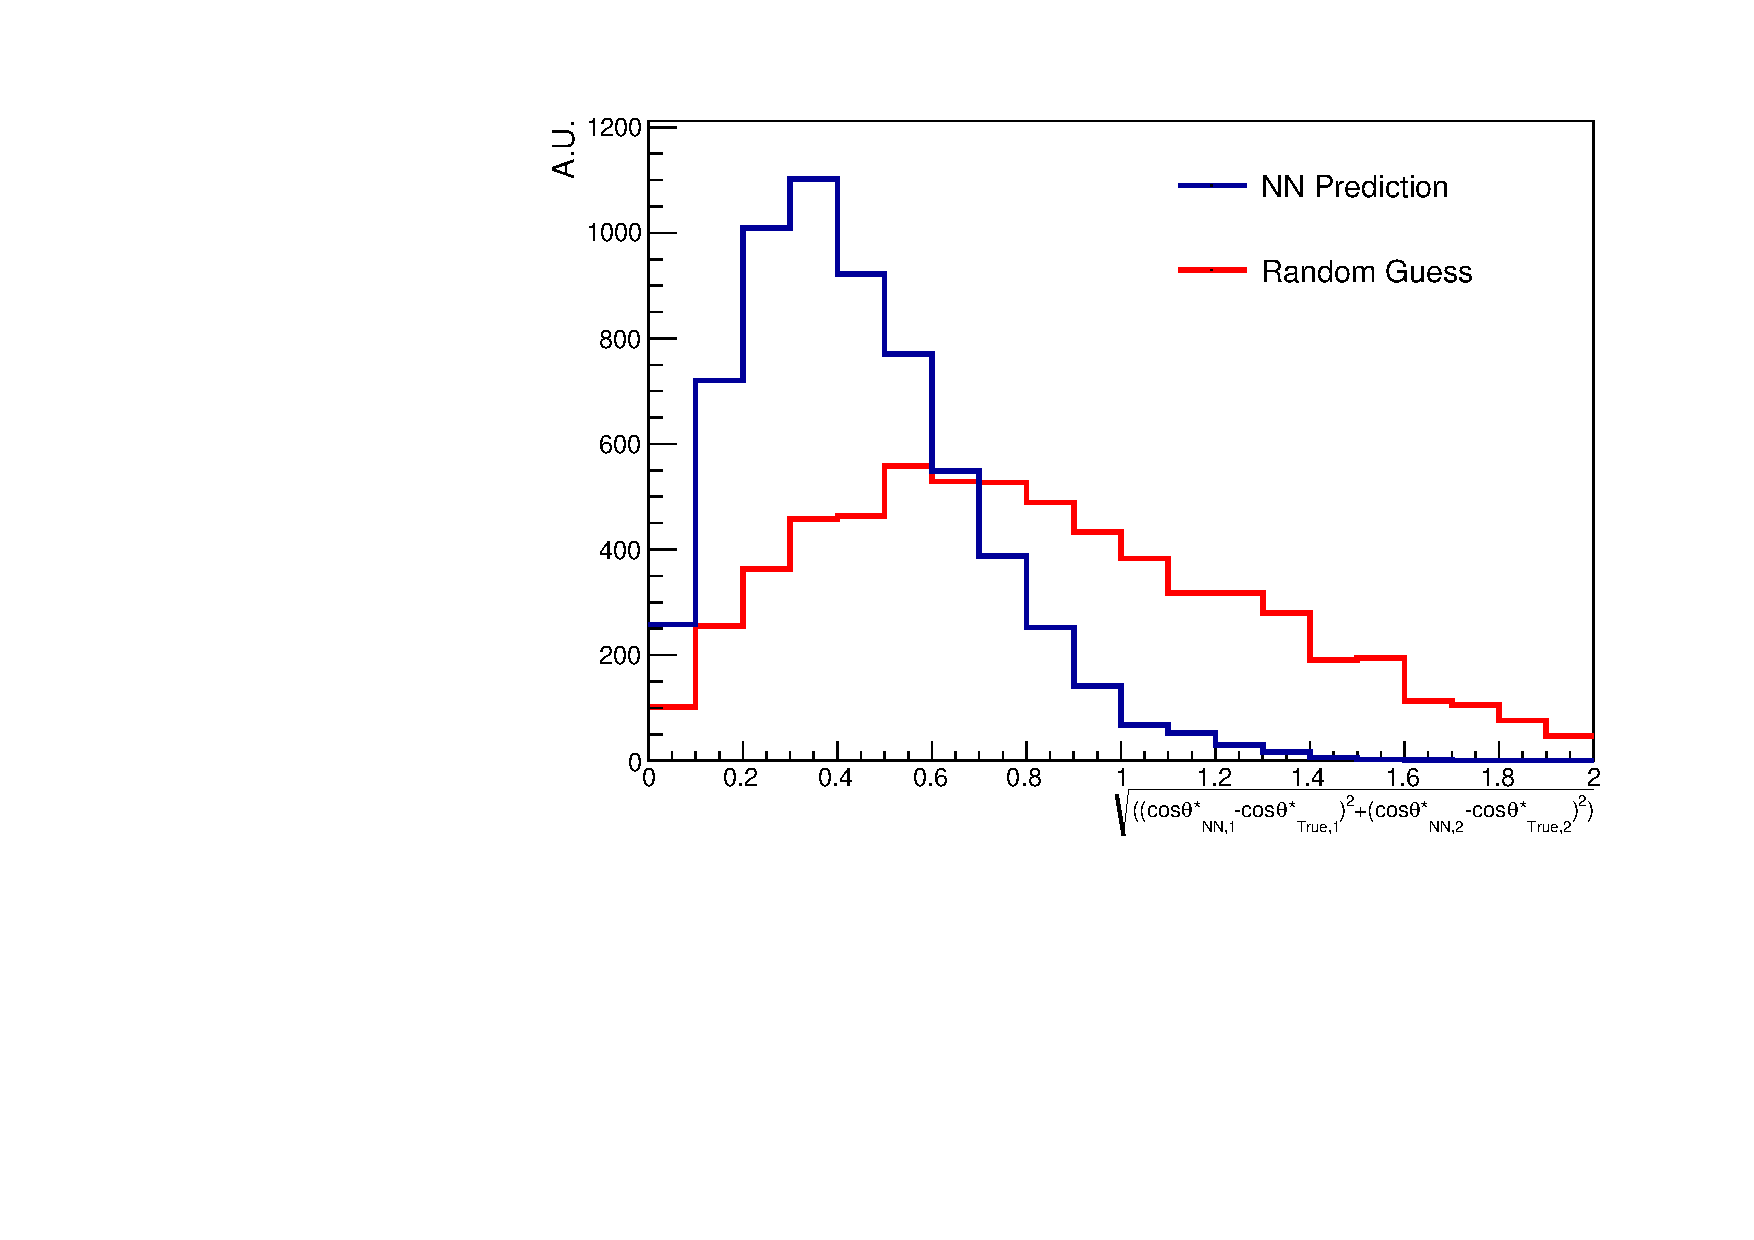
\includegraphics[width=.45\textwidth]{./fig/OneD_cts_compare.pdf}
\caption{\label{fig:mlp_err} Distance of prediction from the true value of ($\ctsnb(1)$,$\ctsnb(2)$)}
\end{figure}







\section{Signal Model}


As our default sample, leading order electroweak-Same sign WW events were produced at parton level with madgraph~\cite{} using nn23l01~\cite{} pdf, and the following generator level cuts. 

\begin{itemize}
\item Parton $p_T > 20$ GeV, $|\eta| < 5$
\item Lepton $p_T > 10$ GeV, $|\eta| < 2.5$
\item $\dR (j,j),\dR (l,l),\dR (l,j) > 0.4$
\item Invariant mass of the two parton system $M(j,j)> 150$ GeV
\end{itemize}

The resulting cross section at $13$ TeV is 8.4 fb$^{-1}$ which is used to normalized the expected number of events.

we will first demonstrate the usefulness of deep learning networks with this general sample, then discuss the effects of cuts to reject other backgrounds as well as detector modeling effects. 

Polarization fractions were obtained on the default sample by fitting the \cts variable determined at truth level. In order to fit for these polarization fractions templates must be built for ``pure'' polarization states. These templates are created by reweighting each event based on the truth \cts distribution. With weights $W_i$ given by

\begin{multline}
W_i = \frac{ F_i }{Norm(\ts_1,\ts_2)}\\
Norm(\ts_1,\ts_2)=[ \frac{3}{8} f_L (1 \mp \ctsnb_1))^2 + \frac{3}{8} f_R (1 \pm \ctsnb_1))^ 2\\ 
+\frac{3}{4} f_0 (1 - \ctsSqnb_1))]  [(\ctsnb_1) \rightarrow \ctsnb_2))] 
\end{multline}

where $F_i$ represents the six possible polarization states for the two W's: Left-Left (LL), Left-Right (LR), Right-Right(RR), Right-Longitudinal (RO), Left-Longitudinal (LO), or Longitudinal-Longitudinal (LO).

\small
\begin{equation}
F_i \in  \left( \begin{array}{c} 
  OO=F_0^2 [(1 - \ctsnb_1))(1 - \ctsnb_2))],\\
  LL=F_L^2 [(1 \mp \ctsnb_1))(1 \mp \ctsnb_2))],\\
  RR=F_R^2 [(1 \pm \ctsnb_1))(1 \pm \ctsnb_2))],\\
  LR=F_L F_R[ (1 \mp \ctsnb_1))(1 \pm \ctsnb_2))\\ \;\;+(1 \mp \ctsnb_2))(1 \pm \ctsnb_1))],\\
  LO=F_L F_O[ (1 \mp \ctsnb_1))(1 - \ctsnb_2))\\  \;\;+(1 \mp \ctsnb_2))(1 - \ctsnb_1)) ],\\
  RO =F_R F_O[ (1 \pm \ctsnb_1))(1 - \ctsnb_2))\\  \;\;+(1 \pm \ctsnb_2))(1 - \ctsnb_1)) ]\\
\end{array} \right)
\end{equation}
\normalsize
Where, since no ordering is applied to the W bosons we  require that the individual polarization fractions $F_L$,$F_R$,$F_0$ are equal for both W's. For reweighting the original sample $F_L$,$F_R$,$F_0$  are take as a function of M(W,W). Weights are calculated before any additional event level cuts are made, and the resulting templates are remade for each set of cuts explored.
 
While there are six possible polarization combinations not all polarization states are as interesting from the the stand point of new physics, and better measurements can be preformed if assumptions can be made. To Illustrate this we define 4 more templates L,R,O,$\slashed{O}\slashed{O}$. L,R,O fit for the number of Left,Right, and Longitudinal W's as would commonly be done in \cts distributions in events with two W's such as in semi-leptonic $t \overline{t}$ events~\cite{}. $\slashed{O}\slashed{O}$ assumes all new physics would be encoded in the longitudinal-longitudinal polarization final state and the only free parameter is the longitudinal-longitudinal fraction.

\small
\begin{equation}
\begin{array}{c}
TT=LL+LR+RR\\
OT=OL+LT\\
\slashed{O}\slashed{O}=LL+RR+LR+LO+RO\\
\end{array}
\end{equation}
\normalsize

In addition the templates are checked by requiring that the fitted values for each fraction match the values obtained a truth level. ~\textcolor{red}{In addition these fractions and kinematics were checked explicitly using Madspin.} In order to compare against other sensitive variables we also apply this reweighting to $R_{pt}$.

\begin{figure}
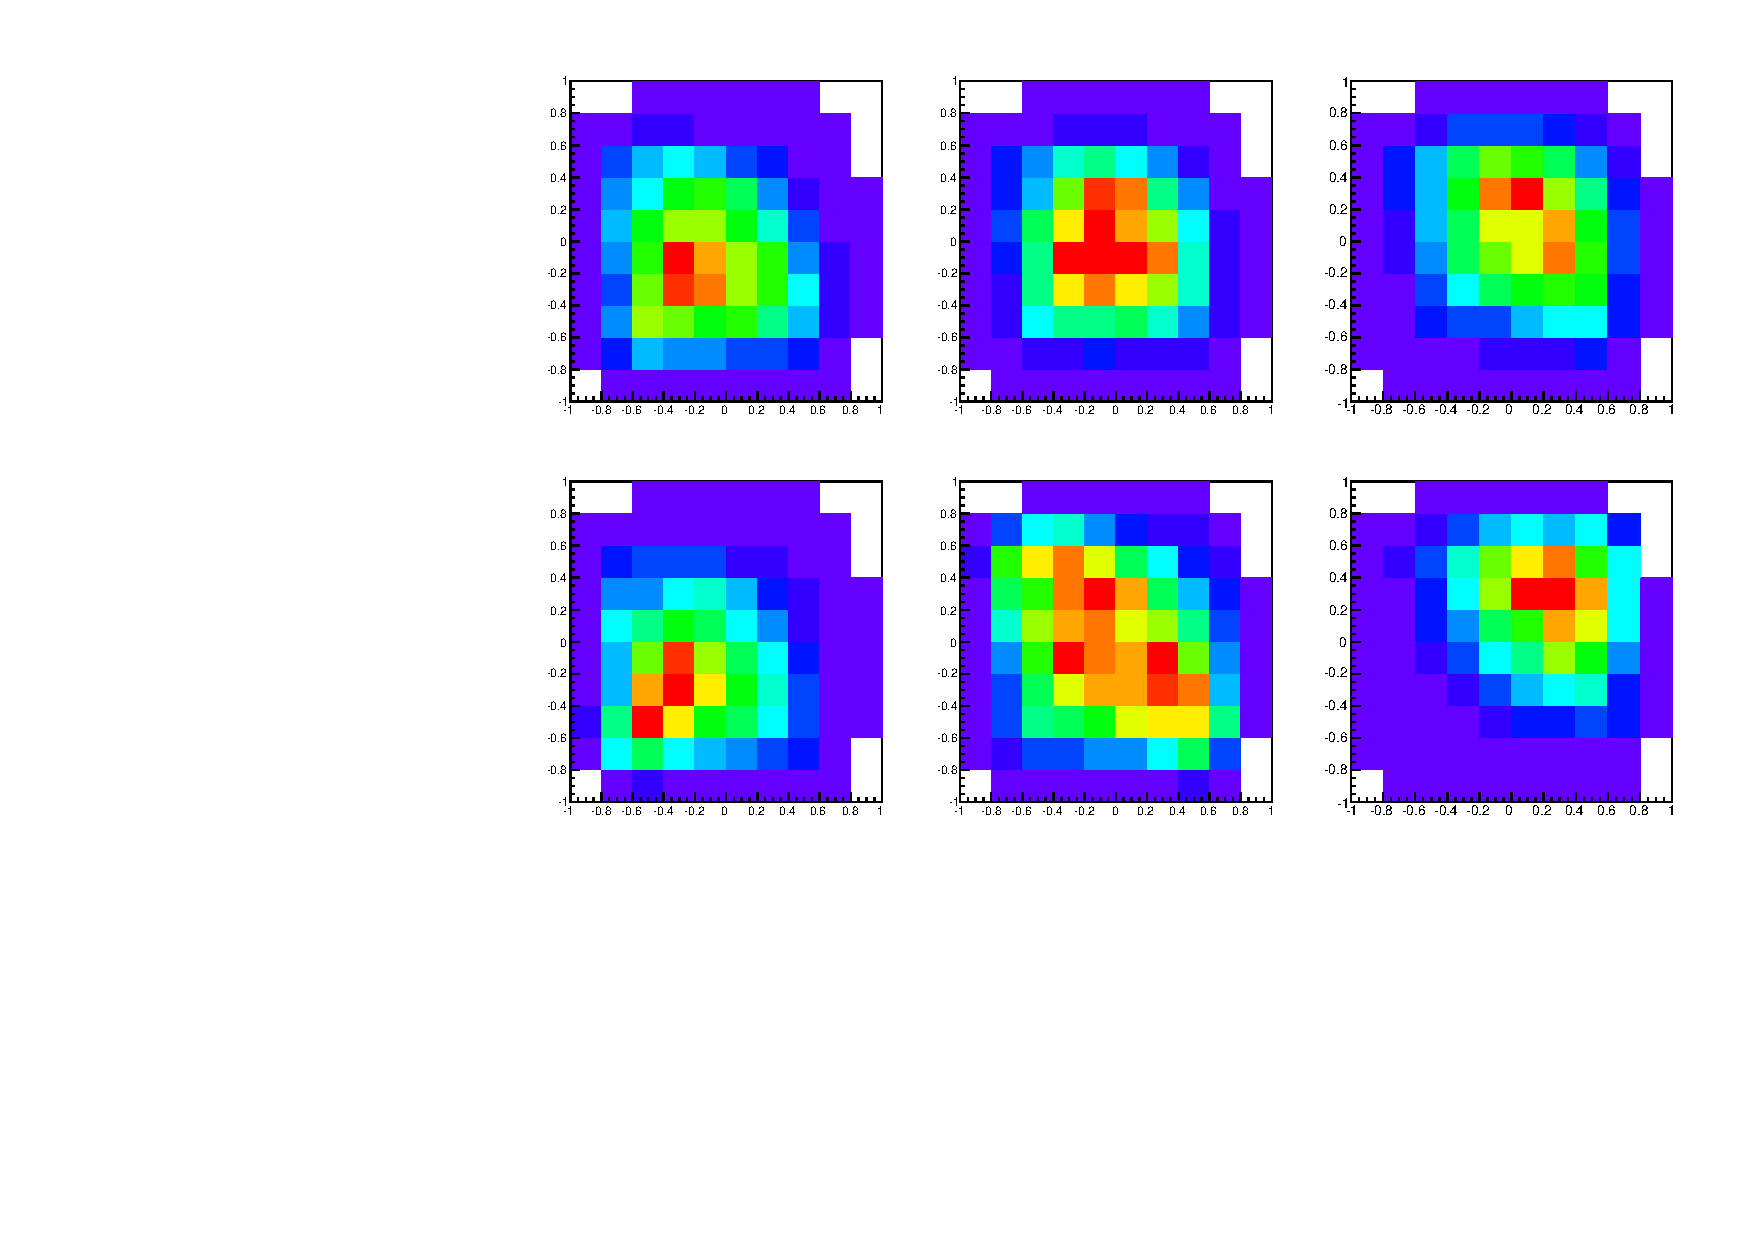
\includegraphics[width=.45\textwidth]{./fig/2D_temps.pdf}

\caption{Two dimensional templates after reweighting to pure polarization states which clock-wise from the upper left LO,OO,RO,LL,LR,RR.
\label{fig:mlp_err} Distance of prediction from the true value of ($\ctsnb(1)$,$\ctsnb(2)$)}
\end{figure}


\begin{figure}
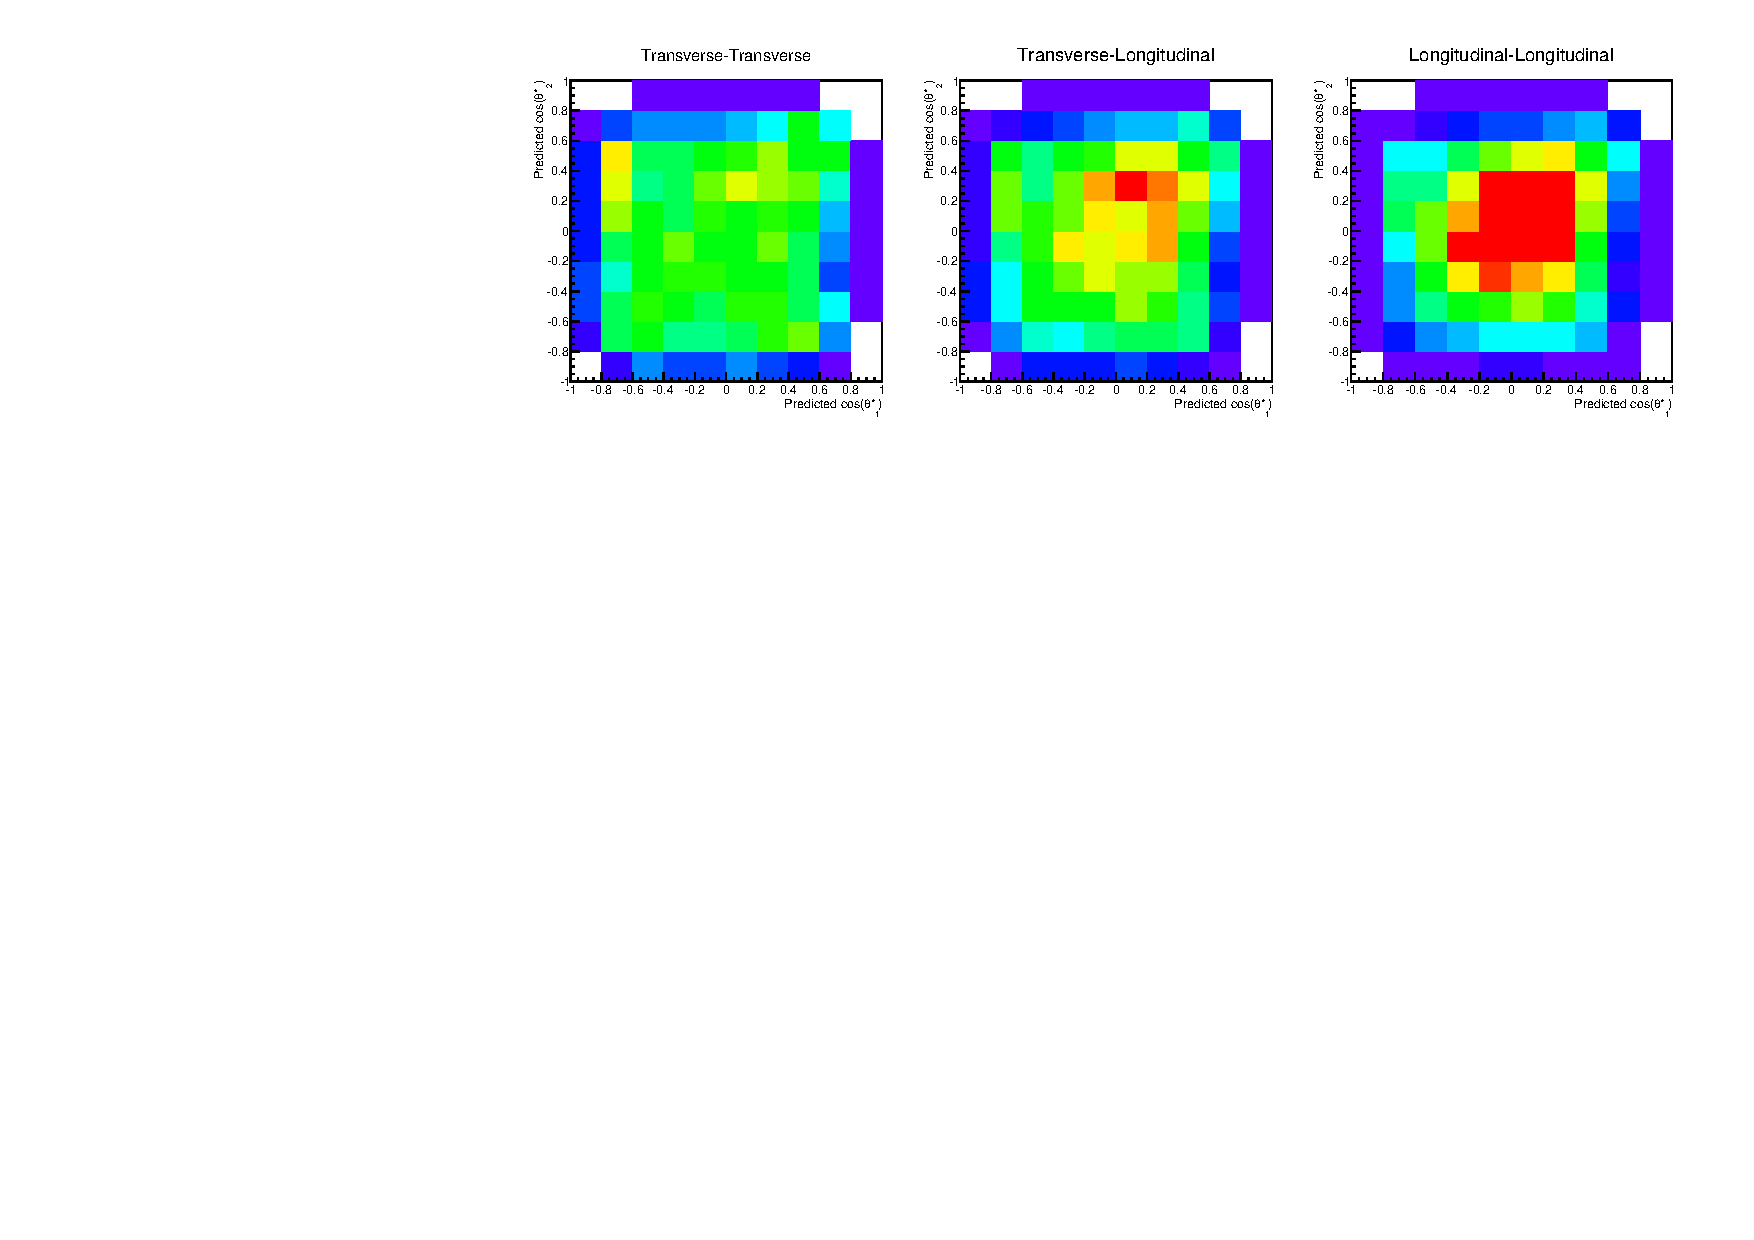
\includegraphics[width=.45\textwidth]{./fig/templates.pdf}
\caption{Templates for Neural Network output }
\end{figure}


\begin{figure}
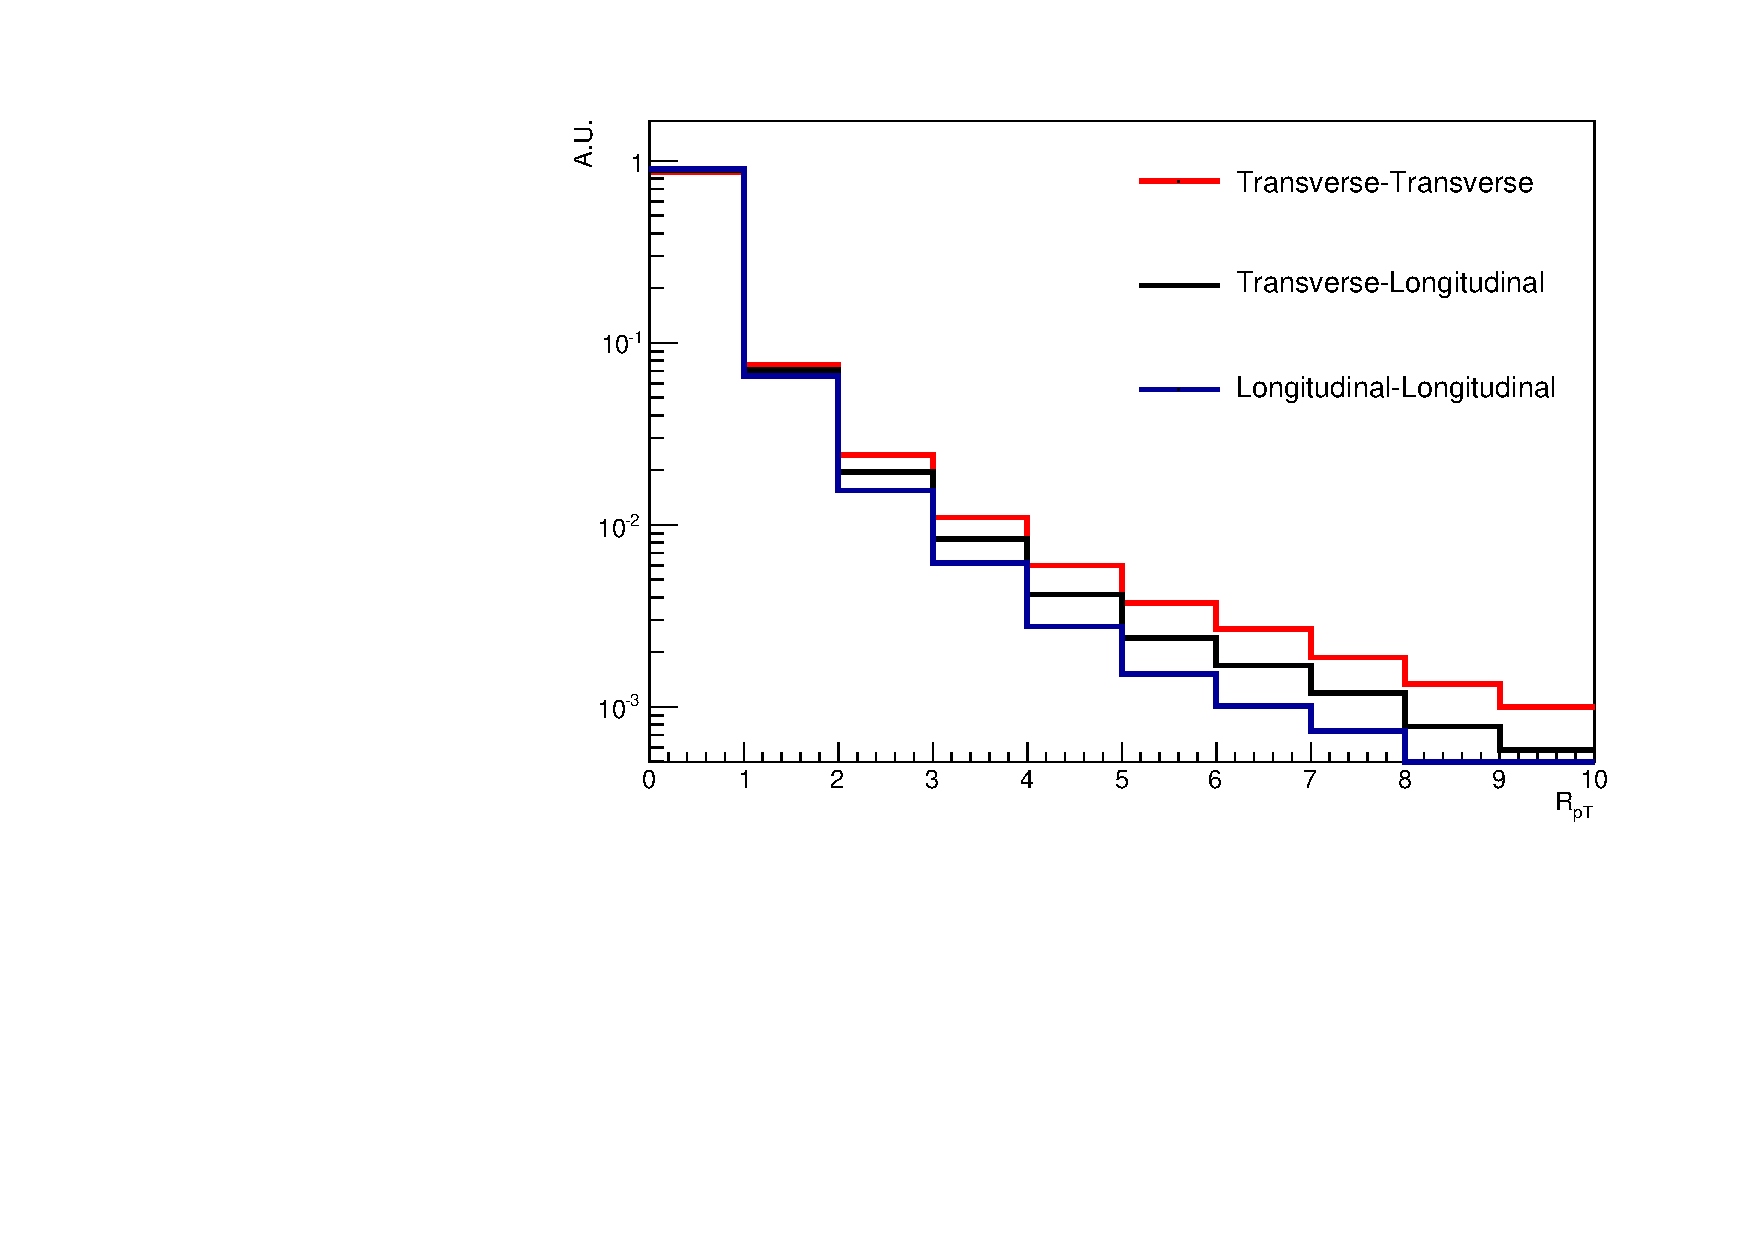
\includegraphics[width=.45\textwidth]{./fig/templates_2D.pdf}
\caption{Templates for $R_{pT}$}
\end{figure}




\section{Predictions for the LHC}

Armed with templates for each polarization state, and a sensitive distribution all we have to do is fit the resulting 2D-Data for each polarization fraction. In actually data analysis, this would involve
first selecting events to remove background, and then subtracting predicted background from data. The effect of additional cuts and backgrounds is covered below, but for the case of this section we assume that 
Madgraph selection can be fit directly to obtain sensitivities. The maximum likelihood fit is preformed with the RooFit~\cite{} frame work. Fit errors were determined by randomly fluctuating data expectations within their Poisson errors and repeating the fit, and confidence intervals were derived from these toy experiments. The precision for various configurations of templates can be seen in Figures~\ref{fig:sen_6,fig:sen_3,fig:sen_2}.  It can be seen that as expected better precision can be obtained by reducing the number of it templates by fixing groups of polarization to the SM prediction. In~\ref{fig:sin_3} that the the Transverse components can be measured we great precision, whereas separating pure longitudinal-longitudinal scattering from longitudinal-transverse scattering is challenging. However, in~\ref{fig:sen_2} shows that fixing the the Transverse-Longitudinal fraction to the SM prediction allows for an excellent extraction of the Longitudinal-Longitudinal fraction from the combination of all others. In all cases the neural network output outperforms $R_{pT}$.


\begin{figure}
Example fit
\end{figure}



\begin{figure}
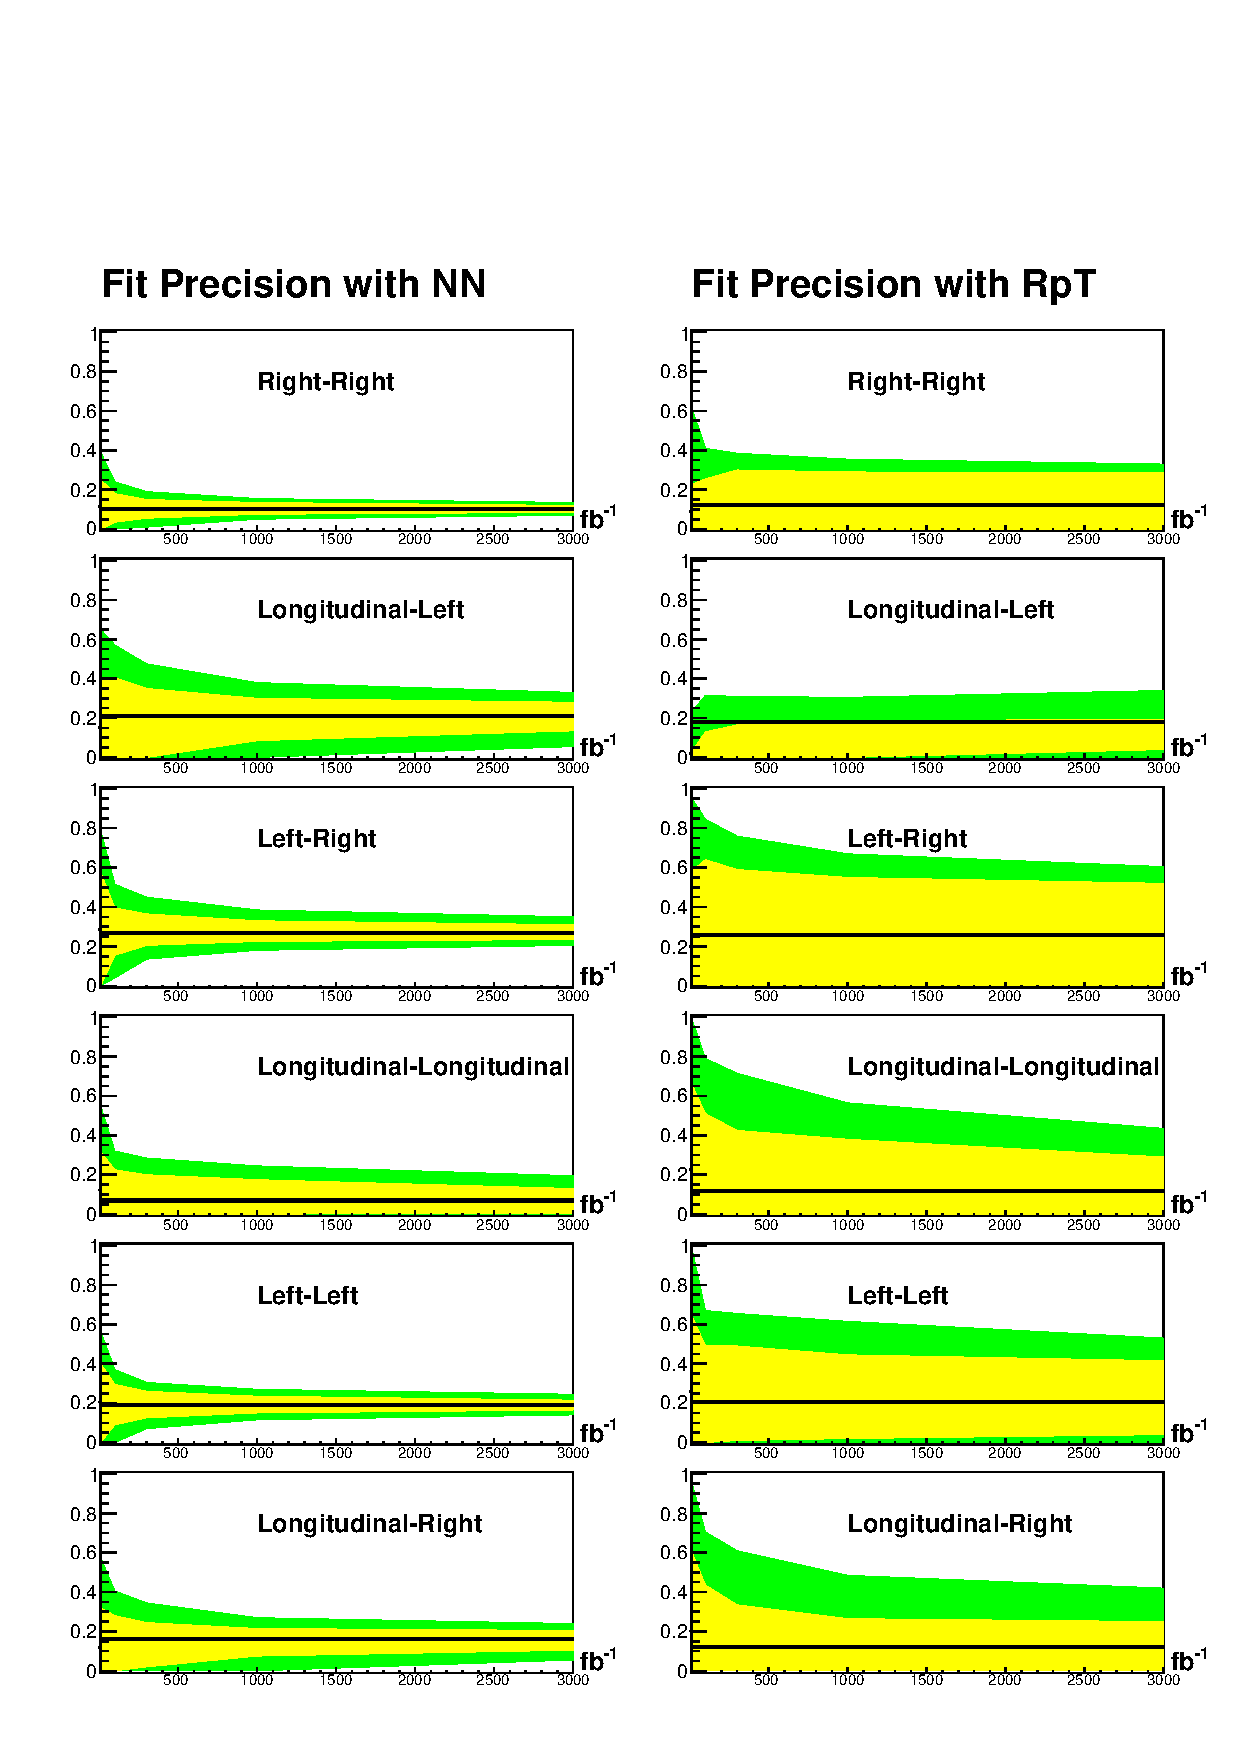
\includegraphics[width=.45\textwidth]{./fig/sens_0.pdf}
\caption{\label{fig:sen_6} 68\% and 95\% confidence intervals for fits with six templates. Fits of the neural network on the right and fits of $R_{pT}$ the on the left}
\end{figure}


\begin{figure}
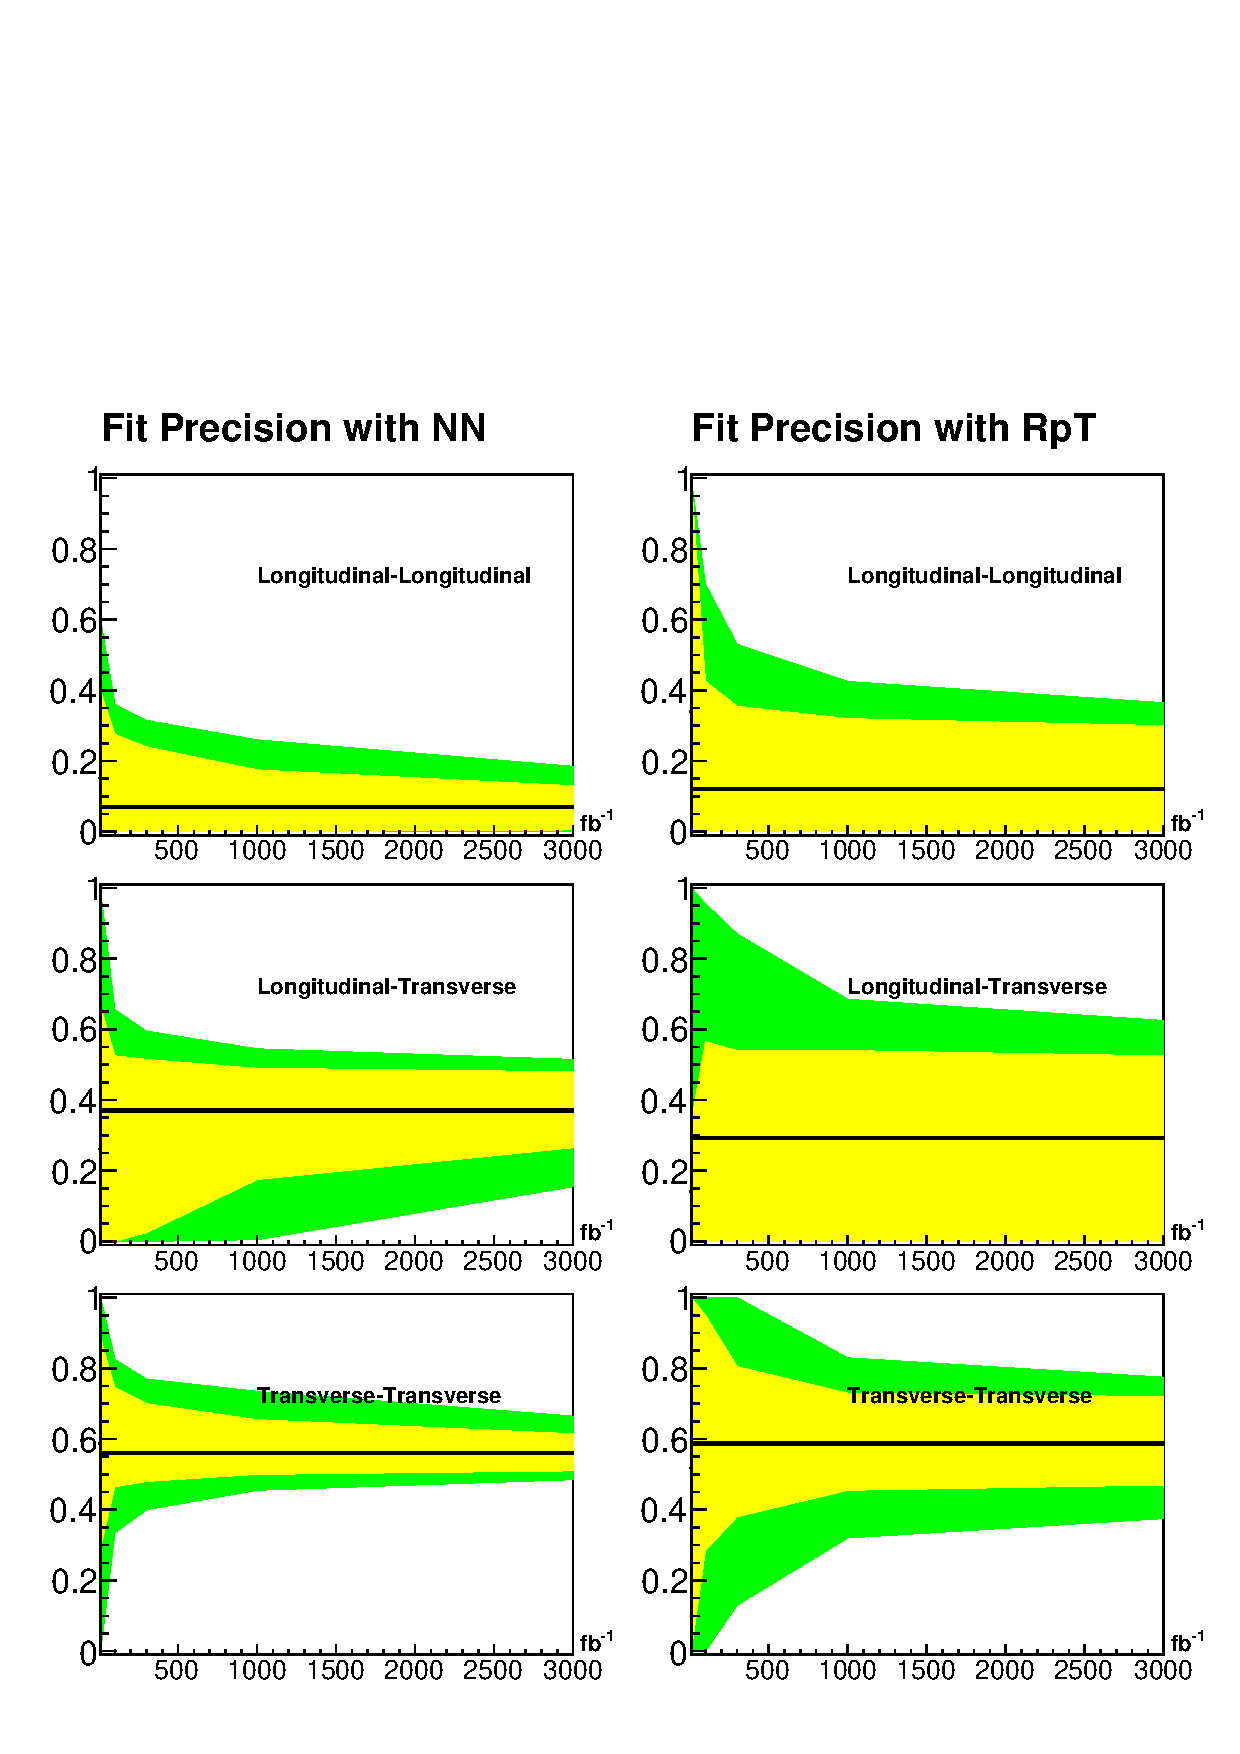
\includegraphics[width=.45\textwidth]{./fig/sens_1.pdf}
\caption{ \label{fig:sen_3} 68\% and 95\% confidence intervals for fits with three templates. Fits of the neural network on the right and fits of $R_{pT}$ the on the left}
\end{figure}


\begin{figure}
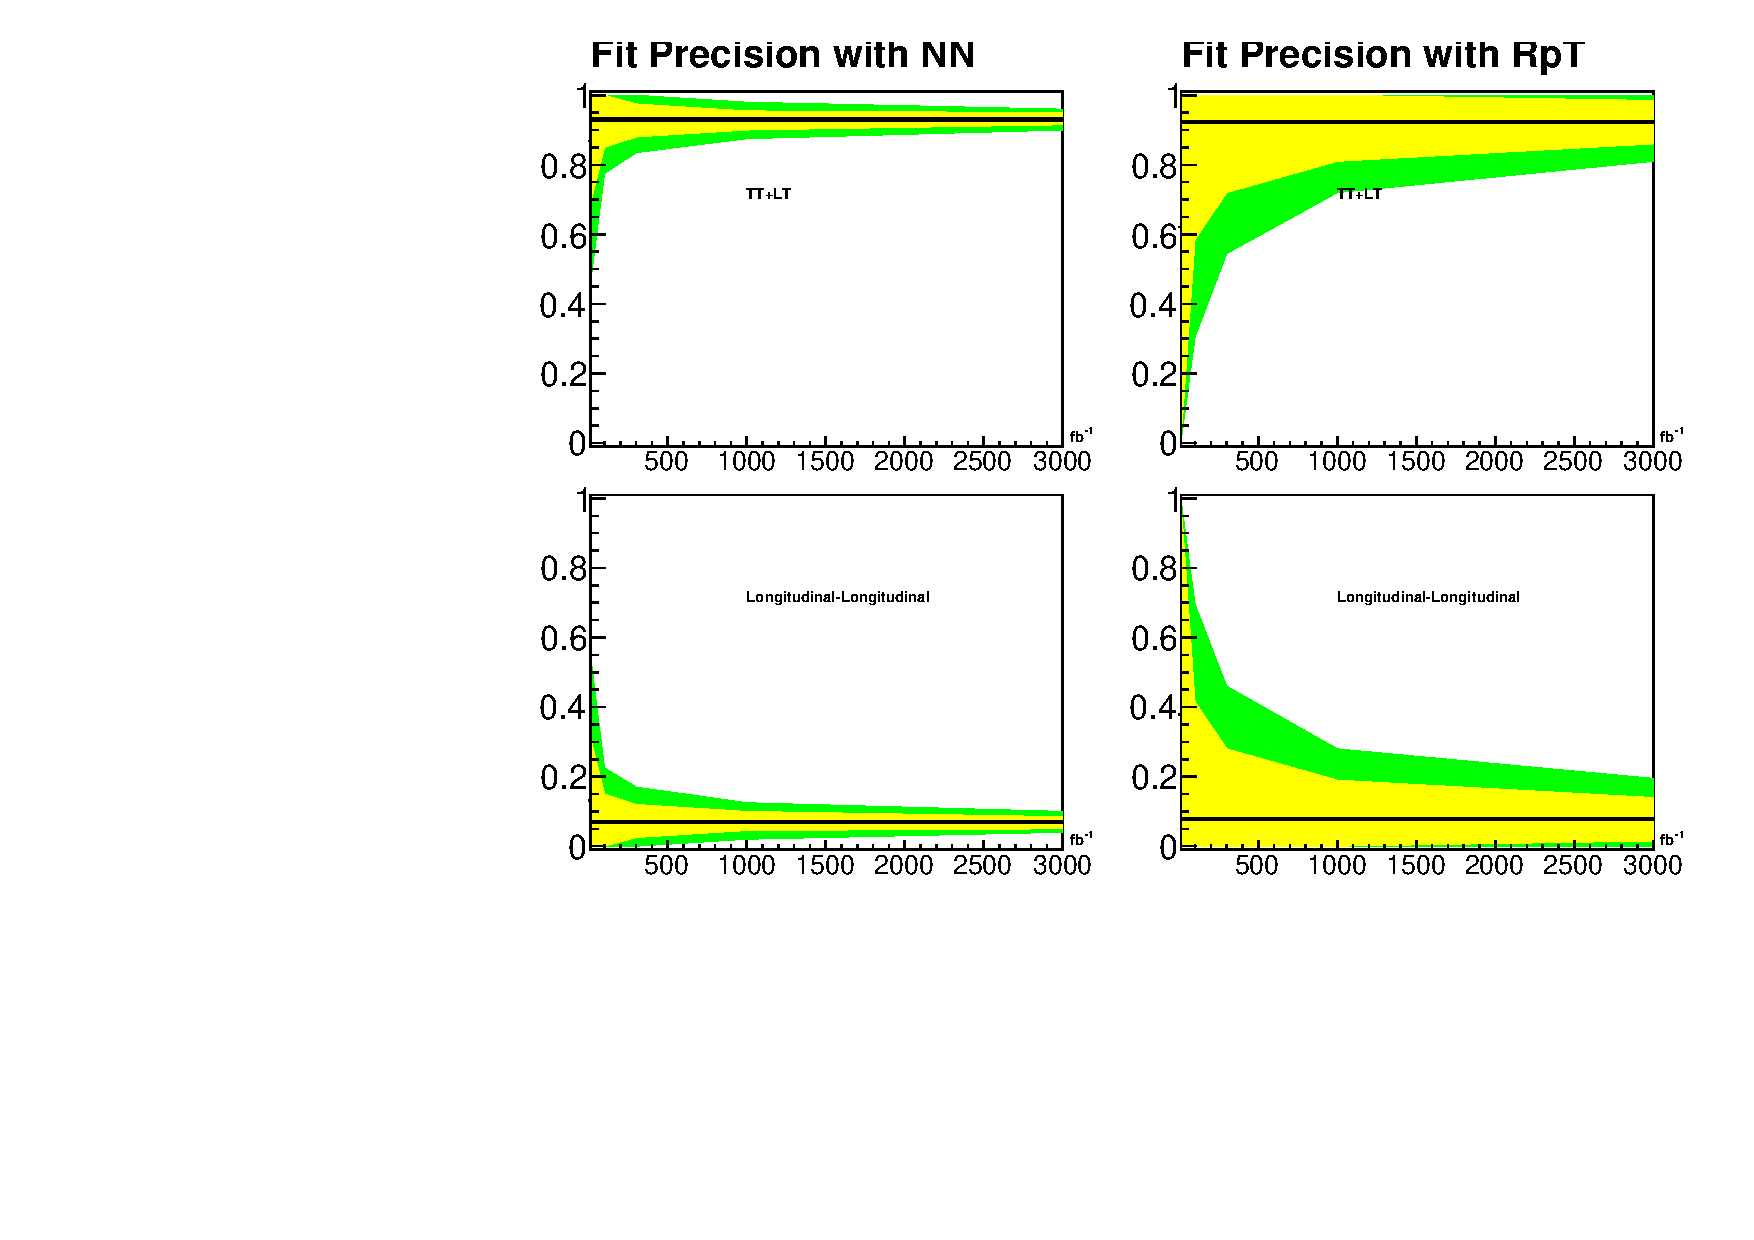
\includegraphics[width=.45\textwidth]{./fig/sens_2.pdf}
\caption{\label{fig:sen_2} 68\% and 95\% confidence intervals for fits with two templates. Fits of the neural network on the right and fits of $R_{pT}$ the on the left}

\end{figure}


\section{Detector Studies}

While the success of this neural network at simple parton level is encouraging, it is important to check if this procedure will stand
up to experimental realities of finite detector resolution, and non \ssWW background. To remove background the ATLAS collaboration applied
the following cuts to a sample of two same sign leptons with two jets.

\begin{itemize}
\item Jet $p_T > 30$ GeV
\item Lepton $p_T > 25$ GeV
\item Lepton $\slashed{E}_T > 40$ GeV
\item $M(j,j) > $500 GeV
\item $\Delta Y(j,j) < 2.4 $
\end{itemize}

After these cuts the dominate background results WZ production. Table~\ref{tab:sens} shows the effect of applying these cuts 
and preforming the same fits at parton level. Additional Table~\ref{tab:sense}, shows the effect of passing the parton level events
through pythia6 for hadronization, and then through Delphes (using the CMS simulation card.) to simulate generic detector smearing. Each additional cut or smearing
decreases the sensitivity to the various polarization components as expected, but the possibility to strongly constrain the VBS polarization remain. Figure~\ref{sig_bkg} shows for comparison the shape produced by the dominant background to ATLAS's \ssWW study. I can be seen that this background closely resembles the RR template, and it will be important for the WZ to be correctly subtracted before the \cts is fitted for polarization fractions.


\begin{figure}
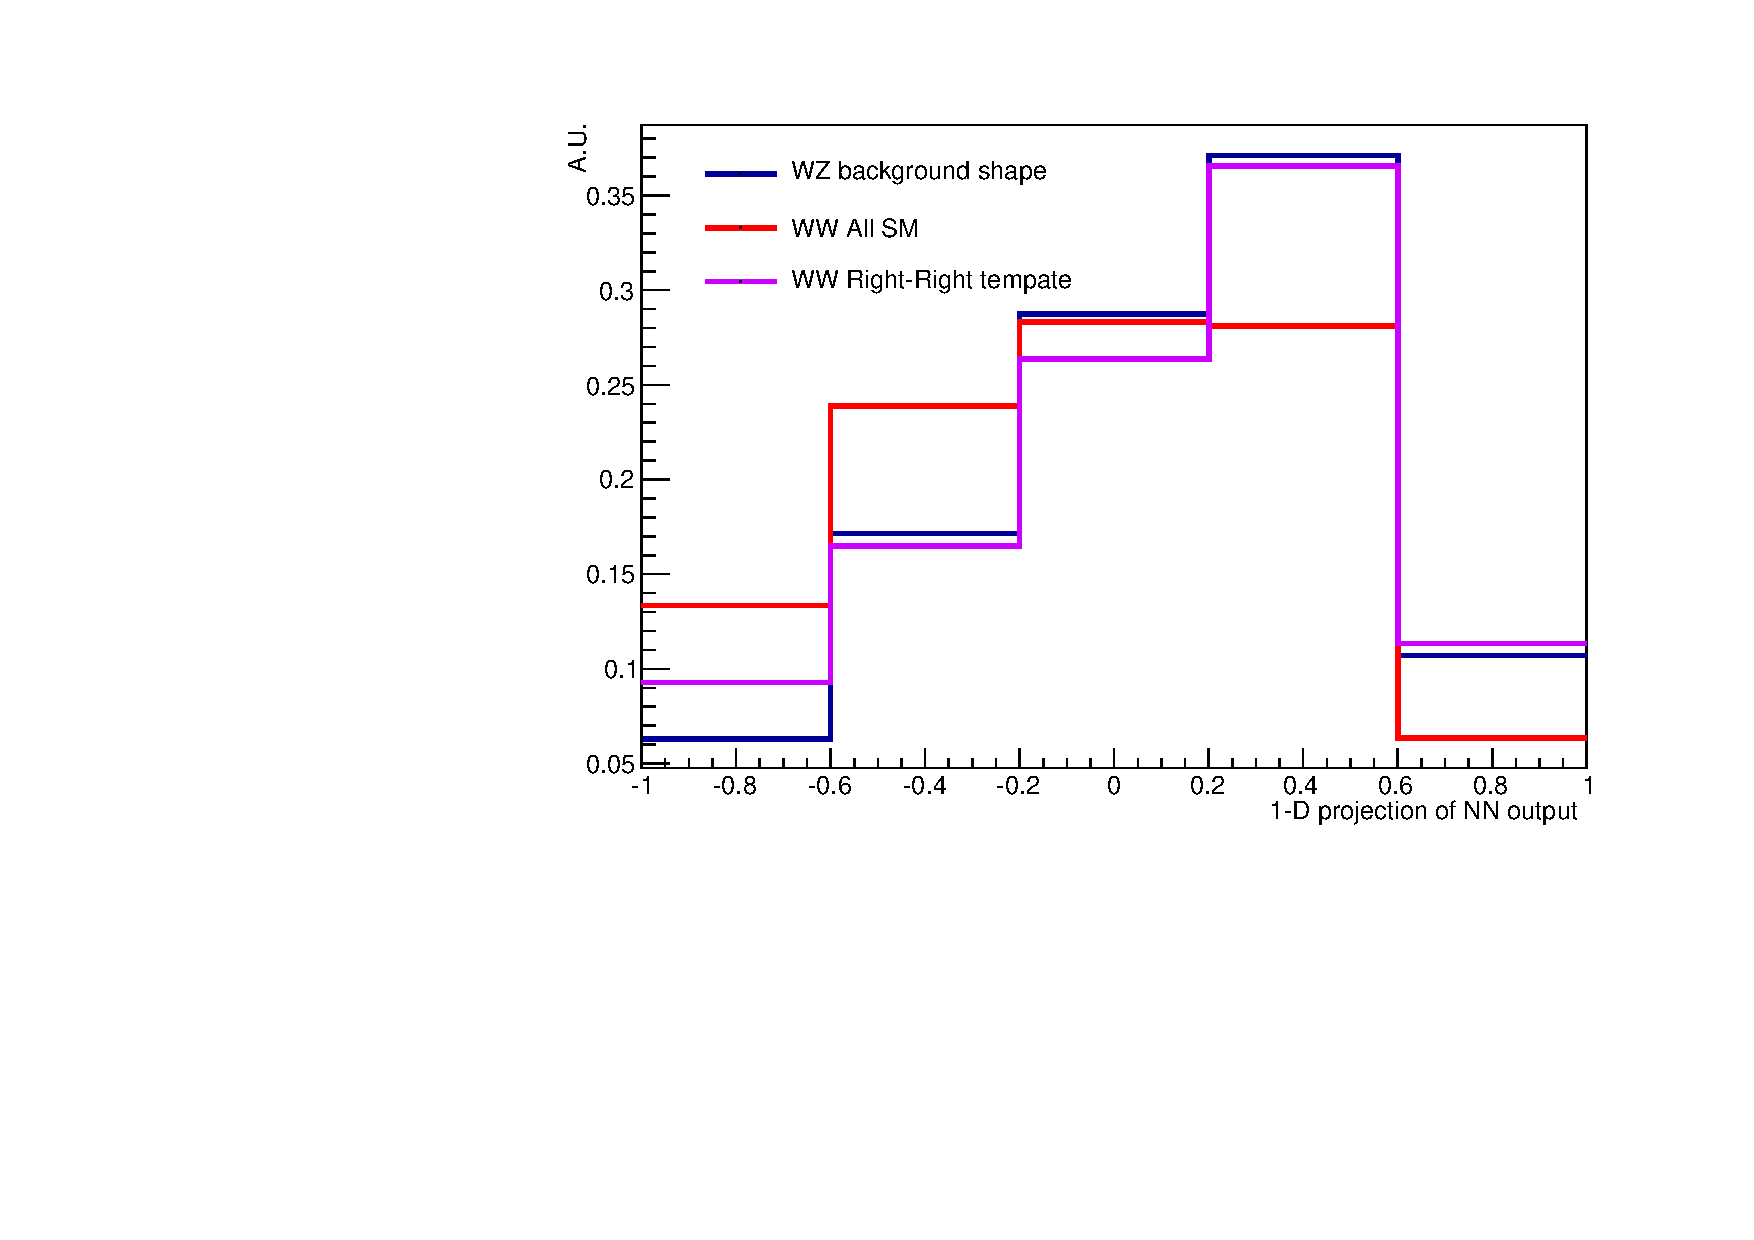
\includegraphics[width=.45\textwidth]{./fig/sig_bkg.pdf}
\caption{\label{sig_bkg} Signal and background shapes}

\end{figure}

 


\section{Conclusions}

We've demonstrated that same sign VBS studies can be used to directly study Longitudinal-Longitudinal bosons scattering in spite
of the missing information resulting for neutrinos. The use of a deep neural network significantly out preforms the benchmark variable
of $R_pT$. Cuts to reject backgrounds as well as detector smearing reduces the sensitivity as expected, but the method remains a useful tool
for the study of VBS.



\begin{table*}[h!]
\begin{center}
\begin{tabular}{c |cc|cc|cc}
\hline
Templates & \multicolumn{2}{c|}{TT} & \multicolumn{2}{c|}{OT}  & \multicolumn{2}{c}{OO} \\
\hline
 & LL & UL & LL & UL & LL & UL  \\
\hline
Parton & 0.51 & 0.62 &0.27 & 0.48 &0.01 & 0.13\\ 
ATLAS Cuts Parton & 0.47 & 0.63 &0.19 & 0.52 &0.0 & 0.19\\ 
Delphes & 0.48 & 0.65 &0.16 & 0.52 &0.0 & 0.21\\ 
ATLAS Cuts Delphes & 0.44 & 0.66 &0.08 & 0.56 &0.0 & 0.27\\ 
\hline
\hline
\end{tabular}
\caption{\label{tab:sens}) Lower Limits (LL) and Upper Limits (UL) for various different simulations.}
\end{center}
\end{table*}

\begin{table}[h!]
\begin{tabular}{c |cc|cc}
\hline
Templates & \multicolumn{2}{c|}{!OO} & \multicolumn{2}{c}{OO} \\
\hline
 & LL & UL & LL & UL  \\
\hline
Parton & 0.92 & 0.95 &0.05 & 0.09\\ 
ATLAS Cuts Parton & 0.89 & 0.95 &0.05 & 0.11\\ 
Delphes & 0.9 & 0.95 &0.05 & 0.11\\ 
ATLAS Cuts Delphes & 0.87 & 0.95 &0.05 & 0.13\\ 
\hline
\hline
\end{tabular}
\caption{ Lower Limits (LL) and Upper Limits (UL) for various different simulations.}
\end{table}

\section{conclusions}


\begin{thebibliography}{99}
%\cite{Chatrchyan:2012ufa}
%\cite{Aad:2012tfa}
\bibitem{ATLAS_higgs} 
  G.~Aad {\it et al.}  [ATLAS Collaboration],
  %``Observation of a new particle in the search for the Standard Model Higgs boson with the ATLAS detector at the LHC,''
  Phys.\ Lett.\ B {\bf 716}, 1 (2012)
  [arXiv:1207.7214 [hep-ex]].
  %%CITATION = ARXIV:1207.7214;%%
  %4423 citations counted in INSPIRE as of 02 Jun 2015


\bibitem{CMS_higgs} 
  S.~Chatrchyan {\it et al.}  [CMS Collaboration],
  %``Observation of a new boson at a mass of 125 GeV with the CMS experiment at the LHC,''
  Phys.\ Lett.\ B {\bf 716}, 30 (2012)
  [arXiv:1207.7235 [hep-ex]].
  %%CITATION = ARXIV:1207.7235;%%
  %4343 citations counted in INSPIRE as of 02 juin 2015

%\cite{Aad:2014zda}
\bibitem{ATLAS_ssWW} 
  G.~Aad {\it et al.}  [ATLAS Collaboration],
  %``Evidence for Electroweak Production of $W^{\pm}W^{\pm}jj$ in $pp$ Collisions at $\sqrt{s}=8$ TeV with the ATLAS Detector,''
  Phys.\ Rev.\ Lett.\  {\bf 113}, no. 14, 141803 (2014)
  [arXiv:1405.6241 [hep-ex]].
  %%CITATION = ARXIV:1405.6241;%%
  %26 citations counted in INSPIRE as of 02 juin 2015


%\cite{Khachatryan:2014sta}
\bibitem{CMS_ssWW} 
  V.~Khachatryan {\it et al.}  [CMS Collaboration],
  %``Study of vector boson scattering and search for new physics in events with two same-sign leptons and two jets,''
  Phys.\ Rev.\ Lett.\  {\bf 114}, no. 5, 051801 (2015)
  [arXiv:1410.6315 [hep-ex]].
  %%CITATION = ARXIV:1410.6315;%%
  %6 citations counted in INSPIRE as of 02 juin 2015


%\cite{Han:2009em}
\bibitem{Han:2009em} 
  T.~Han, D.~Krohn, L.~T.~Wang and W.~Zhu,
  %``New Physics Signals in Longitudinal Gauge Boson Scattering at the LHC,''
  JHEP {\bf 1003}, 082 (2010)
  [arXiv:0911.3656 [hep-ph]].
  %%CITATION = ARXIV:0911.3656;%%
  %38 citations counted in INSPIRE as of 02 juin 2015

%\cite{Doroba:2012pd}
\bibitem{Doroba:2012pd} 
  K.~Doroba, J.~Kalinowski, J.~Kuczmarski, S.~Pokorski, J.~Rosiek, M.~Szleper and S.~Tkaczyk,
  %``The $W_L W_L$ Scattering at the LHC: Improving the Selection Criteria,''
  Phys.\ Rev.\ D {\bf 86}, 036011 (2012)
  [arXiv:1201.2768 [hep-ph]].
  %%CITATION = ARXIV:1201.2768;%%
  %11 citations counted in INSPIRE as of 02 juin 2015



%\cite{Baldi:2014kfa}
\bibitem{Baldi:2014kfa} 
  P.~Baldi, P.~Sadowski and D.~Whiteson,
  %``Searching for Exotic Particles in High-Energy Physics with Deep Learning,''
  Nature Commun.\  {\bf 5}, 4308 (2014)
  [arXiv:1402.4735 [hep-ph]].
  %%CITATION = ARXIV:1402.4735;%%
  %2 citations counted in INSPIRE as of 02 juin 2015

%\cite{Baldi:2014pta}
\bibitem{Baldi:2014pta} 
  P.~Baldi, P.~Sadowski and D.~Whiteson,
  %``Enhanced Higgs Boson to $\tau^+\tau^-$ Search with Deep Learning,''
  Phys.\ Rev.\ Lett.\  {\bf 114}, no. 11, 111801 (2015)
  [arXiv:1410.3469 [hep-ph]].
  %%CITATION = ARXIV:1410.3469;%%

\end{thebibliography}


\end{document}
